%\documentclass[12pt,letterpaper,doublespaced,ETD,dvips]{gt-ece-thesis}
\documentclass[12pt,letterpaper,doublespaced,ETD]{gt-ece-thesis} %taking dvips out enable pdf bookmark generation as well as the logo printing on the first page

\title{Multi-Target Tracking Using Residual Vector Quantization}
\author{Salman Aslam}
\copyrightyear{2010}
\graddate{December 2010}  
\approvaldate{December 2010}  

\addadvisor{Dr. Christopher F. Barnes}{Asst. Professor, School of ECE}{Georgia Institute of Technology}
\addchair{Dr. David V. Anderson}{Professor, School of ECE}{Georgia Institute of Technology}
\addreader{Dr. Aaron F. Bobick, Co-advisor}{Professor, School of Interactive Computing}{Georgia Institute of Technology}
\addreader{Dr. Vijay Madisetti}{Asst. Professor, School of ECE}{Georgia Institute of Technology}
\addreader{Dr. Patricio Vela}{Asst. Professor, School of ECE}{Georgia Institute of Technology}



\bibfiles{c:/salman/work/writing/MyCitations}

\titlepagetrue
\figurespagetrue
\tablespagetrue
\contentspagetrue
\symbolspagefalse
\glossarypagefalse 
\bibpagetrue
\mastersthesisfalse 
\multivolumefalse
\singlespacednotestrue


\usepackage{graphicx, subfigure}
\usepackage{insfig}
\usepackage{url}
\usepackage{multirow}
\usepackage{hyperref}
\usepackage{longtable}
\usepackage{color}

\setchaptertocdepth{2}
\setappendixtocdepth{2}

\settocstring{Table of Contents}
\setlofstring{List of Figures}
%\setlotstring{List of Tables}
\setbibstring{References}
\setindstring{Index}
\setdedstring{Dedication}
\setglostring{List of Terms}
\setchpstring{Chapter}
\setappstring{Appendix}
\setprtstring{Volume}
\setabsstring{Summary}
\setlosstring{List of Symbols}
\setackstring{Acknowledgment}

\setfrontpagestyle{plain}
\setbodypagestyle{plain}
\setendpagestyle{plain}

\definecolor{darkgreen}{rgb}{0,0.5,0}
\newcommand{\Ntrg}{\big[N_{t=1, m=1} + \lambda \big] + \big[N_{t=1, m=2} + \lambda \big] + \ldots + \big[N_{t=1, m=M} + \lambda \big]}
\newcommand{\jointcnt}{\sum\limits_{n_{trg}=1}^{N_{trg}}I(X_t=x_t, X_{t-1}=x_{t-1})}
\newcommand{\singlecnt}{\sum\limits_{n_{trg}=1}^{N_{trg}}I(X_{t-1}=x_{t-1})}
\newcommand{\singlep}{p(X_{t-1}=x_{t-1})}
\newcommand{\singlepone}{p(X_{t-1}=1)}
\newcommand{\singleptwo}{p(X_{t-1}=2)}
\newcommand{\singlepM}{p(X_{t-1}=M)}
\newcommand{\condp}{p(X_t=x_t | X_{t-1}=x_{t-1})}
\newcommand{\jointp}{p(X_t=x_t, X_{t-1}=x_{t-1})}
\newcommand{\KmeansOuterSum}{\sum\limits_{k=1}^K}
\newcommand{\KmeansInnerSum}{\sum\limits_{{i=1 \atop x_i \in \mathcal{K}_k}}^N}
\newcommand{\KmeansSum}{\KmeansOuterSum \KmeansInnerSum}
\newcommand{\RVQInnerSum}{\sum\limits_{{i=1 \atop g_i \mapsto m_{\tau, s}}}^N}
\newcommand{\RVQOuterSum}{\sum_{s=1}^S}
\newcommand{\RVQsum}{\KmeansOuterSum \sum\limits_{{i=1 \atop g_i \in \mathcal{K}_k}}^N}
\newcommand{\KmeansInner}{{(x_i - \mu_k)}^2}
\newcommand{\RVQinner}{            {(x_i  - \hat{\mu}^{(k)})}^2}
\newcommand{\RVQinneralternate}{{(g_i - m_\tau^{(k)})}^2}
\newcommand{\RVQinneralternatealternate}{{(g_i - m_{\tau, s})}^2}
\newcommand{\KmeansError}{\KmeansSum \KmeansInner}
\newcommand{\RVQerror}     {\KmeansSum \RVQinner}
\newcommand{\RVQerroralternate}{\RVQsum \RVQinneralternate}
\newcommand{\RVQunit}{x_i -\bigg(\sum_{t=1}^Tm^{(k)}_t\bigg)}
\newcommand{\RVQequivalentCodevector}{\sum_{t=1 }^Tm^{(k)}_t}
\newcommand{\RVQequivalentCodevectorBroken}{\sum_{t=1 \atop t \neq \tau}^Tm^{(k)}_t+ m^{(k)}_\tau}
\newcommand{\RVQmultipleKmeans}{x_i -\bigg(\RVQequivalentCodevectorBroken\bigg)}
\newcommand{\RVQmultipleKmeansone}{x_i -\sum_{t=2}^Tm^{(k)}_t+ m^{(k)}_1\bigg)}
\newcommand{\RVQmultipleKmeansonealternate}{\bigg(x_i -\sum_{t=1 \atop t \neq \tau}^Tm^{(k)}_t\bigg) - m^{(k)}_\tau}
\newcommand{\RVQmultipleKmeanstwo}{x_i -\bigg(\sum_{t=1 \atop t \neq 2}^Tm^{(k)}_t+ m^{(k)}_2\bigg)}
\newcommand{\RVQmultipleKmeansT}{x_i -\bigg(\sum_{t=1}^{T-1}m^{(k)}_t+ m^{(k)}_2\bigg)}
\newcommand{\EucMatrix}
{
\left[
\begin{array}{lll}
r_{11} & r_{12} & t_x \\ 
r_{21} & r_{22} & t_y \\ 
0 & 0 & 1 \\ 
\end{array}
\right]
}	

\newcommand{\SimMatrix}
{
\left[
\begin{array}{lll}
sr_{11} & sr_{12} & t_x \\ 
sr_{21} & sr_{22} & t_y \\
0 & 0 & 1 \\ 
\end{array}
\right]
}

\newcommand{\AffMatrix}
{
\left[
\begin{array}{lll}
a &b & t_x \\ 
c & d & t_y \\
0 & 0 & 1 \\
\end{array}
\right]
}

\newcommand{\ProjMatrix}
{
\left[
\begin{array}{lll}
h_{11} & h_{12} & h_{13} \\ 
h_{21} & h_{22} & h_{23} \\ 
h_{31} & h_{32} & h_{33} \\ 
\end{array}
\right]
}

\newcommand{\RotMatrixTheta}
{
\left[
\begin{array}{rr}
\cos(\theta) & -\sin(\theta) \\ 
\sin(\theta) & \cos(\theta) \\ 
\end{array}
\right]
}

\newcommand{\RotMatrixPhi}
{
\left[
\begin{array}{rr}
\cos(\phi) & -\sin(\phi) \\ 
\sin(\phi) & \cos(\phi) \\ 
\end{array}
\right]
}

\newcommand{\RotMatrixminusPhi}
{
\left[
\begin{array}{rr}
\cos(-\phi) & -\sin(-\phi) \\ 
\sin(-\phi) & \cos(-\phi) \\ 
\end{array}
\right]
}


\newcommand{\EigenvalueMatrix}
{
\left[
\begin{array}{cc}
\lambda_1 & 0\\
0 & \lambda_2
\end{array}
\right]
}

\newcommand{\bigMatrix}
{
s \left[
\begin{array}{cc}
 (r)(a) + b &  (r)(d) - c \\
 (r)(c) - d &  (r)(b) + a
\end{array}
\right]
}


\newcommand{\bigMatrixTwo}
{
\left[
\begin{array}{cc}
(\lambda_2) p + (\lambda_1) q & (\lambda_2) s  - (\lambda_1) r \\
(\lambda_2) r  - (\lambda_1) s & (\lambda_2) q + (\lambda_1) p
\end{array}
\right]
}
\newcommand{\dr}{(\mathbf{x}_i-\boldsymbol\mu_k)^T(\mathbf{x}_i-\boldsymbol\mu_k) + \lambda({Q_{\textrm{max}}-Q_i})}

\begin{document}
	
	\pagestyle{plain}
	\bibliographystyle{ieeetr}

	\begin{FrontMatter}
		\contents %Generates the TOC, LOF, and LOT
	\end{FrontMatter}
	\begin{dedication}
		To my parents, my wife, and my children
	\end{dedication}
	\begin{acknowledgement}
		Thanks to all \newpage
	\end{acknowledgement}
	%\begin{preface}
	%	hello
	%\end{preface}
	\begin{Body}	
		
%@@@@@@@@@@@@@@@@@@@@@@@@@@@@@@@@@@@@@@@@@@@@@@@@@@
\chapter{Introduction}
\label{chap_Introduction}	
%@@@@@@@@@@@@@@@@@@@@@@@@@@@@@@@@@@@@@@@@@@@@@@@@@@
\par
Images have fascinated humans for thousands of years.  The earliest cave paintings have been dated back to around 30,000 years \cite{2009_WEB_EarliestHumanPaintings_Gray}.  Currently, several fields 




%@@@@@@@@@@@@@@@@@@@@@@@@@@@@@@@@@@@@@@@@@@@@@@@@@@
\chapter{Tracking methods}
\label{chap_tracking_methods}	
%@@@@@@@@@@@@@@@@@@@@@@@@@@@@@@@@@@@@@@@@@@@@@@@@@@
%#######################		
\section{Introduction}
%#######################
The biggest challenge in tracking is difficulty in handling changes in target appearance \cite{2008_JNL_subspaceTRK_Ross}.  Intrinsic variations include changes in 

\begin{itemize}
\item pose variation
\item shape deformations
\end{itemize} 

Extrinsic variations include

\begin{itemize}
\item illumination change
\item camera motion
\item camera viewpoint 
\item occlusions
\end{itemize}

An adaptive subspace representation has several advantages:

\begin{itemize}
\item \textbf{Compact representation}.  A subspace represenation using say PCA or RVQ allows storage of a few basis eigenvectors or stage codevectors to capture variations in the target appearance.
\item \textbf{Object recognition}.  This method facilitates object recognition since an appearance model is built for each target.
\item \textbf{Continuous model update}.  As mentioned earlier, changes in target appearance are a big challenge in target tracking.  Online model updating allows the target appearance to be built dynamically.
\item \textbf{Less offline training data required}.  In many instances, few training examples are available that have the same distribution as the expected tracking scenario.  Systems that rely on offline training ignore the information available during online tracking.  An adaptive subspace representation can be used effectively in these scenarios since models are built and maintained online.
\item \textbf{No optimization}.  No complex optimization is required.
\item \textbf{Camera motion}.  This representation does not depend on background maintenance and can therefore be used with moving cameras.
\end{itemize}

%#######################		
\newpage
\section{Affine Warping}
%#######################
%The particle filter generates $N_p$ particles.  However, not carrying the confidence parameter from frame to frame causes the detected target to move around in brownian motion.
%
%Let's say $N_p = 3$ then repmat(rand(1,Np),[Np,1]) gives
%
%\begin{equation*}
%\left[
%\begin{array}{lllll}
%    0.4301  &  0.5482  &  0.8934\\
%    0.4301  &  0.5482  &  0.8934\\
%    0.4301  &  0.5482  &  0.8934\\
%\end{array}
%\right]
%\end{equation*}


\section{2D affine transformation}
\begin{table}[htp]
\centering
\begin{tabular}{| l | c | c | p{2.5in} |}
\hline
Transformation & DoF & Matrix & Distortion\\ \hline 
& & & \\ Projective & 8 & $\ProjMatrix$ & any arbitrary quadrilateral as long as no three points are collinear\\  & & & \\ \hline
& & & \\ Affine & 6 & $\AffMatrix$ & rotation and non-isotropic scaling\\  & & & \\ \hline
& & & \\ Similarity & 5 & $\SimMatrix$ & scaling and rigid motion\\  & & & \\ \hline
& & & \\ Euclidean & 4 & $\EucMatrix$ & rigid motion (rotation, translation) \\  & & & \\ \hline
\end{tabular}\
\caption{2D transformations}
\label{table:2Dtransformations}
\end{table}


Table \ref{table:2Dtransformations} shows different kinds of 2D linear transformations.  Every transformation generalizes the transformation below it in the table.  In this work, we use the 2D affine transform since it is flexible enough to account for most distortions in real images.  However, it cannot handle perspective effects, for which a projective transformation is required. The affine transform is given by,

\begin{equation}
\begin{array}{cccc}
\mathbf{\acute{x}} &=& \mathbf{A}\mathbf{x} + \mathbf{t}\\\\
&=&\mathbf{H}_A \mathbf{x}\\\\
&=& \left[\begin{array}{cccc}\mathbf{A} & \mathbf{t}\\\mathbf{0}^T & 1\end{array}\right] \mathbf{x}\\\\
\left[\begin{array}{l}\acute{x}\\\acute{y}\\1\end{array}\right]   &=& \AffMatrix \left[\begin{array}{l}x\\y\\1\end{array}\right]
\end{array}
\end{equation}

$t_x$ and $t_y$ are translations in the $x$ and $y$ directions respectively.  Including these 2 parameters in $\mathbf{H}_A$ allows the affine transformation to be expressed as a single matrix multiply.  

\subsection{Affine decomposition}
The affine matrix $\mathbf{A}$ can always be decomposed using the SVD decomposition as the product of orthogonal matrices $\mathbf{U}$ and $\mathbf{V}$ and a diagonal matrix $\mathbf{S}$, \cite{2004_BOOK_CG_Hartley}:

\begin{equation}
\begin{array}{llllllll}
\mathbf{A} &= \left[\begin{array}{lll}a_{11} & a_{12} \\ a_{21} & a_{22}\\ \end{array}\right] \\\\
&=\mathbf{U}{\color{blue}\mathbf{S}}\mathbf{V}^t \\\\
&={\color{red}(\mathbf{U}\mathbf{V}^t)}\mathbf{V}{\color{blue}\mathbf{S}}\mathbf{V}^t\\\\
&={\color{red}\mathbf{R}(\theta)}\mathbf{R}(-\phi){\color{blue}\mathbf{S}}\mathbf{R} (\phi)\\\\
&={\color{red}\RotMatrixTheta}\RotMatrixminusPhi{\color{blue}\EigenvalueMatrix}\RotMatrixPhi\\\\
\end{array}
\label{Eq:AffineDecomposition}
\end{equation}

The affine matrix $\mathbf{A}$ can therefore be viewed as a succession of the following 4 steps:

\begin{enumerate} 
\item Rotation by angle $\phi$ 
\item This rotation is followed by a scaling of $\lambda_1$ and $\lambda_2$ in the rotated $x$ and $y$ directions
\item A rotation by angle -$\phi$ which brings the scaled object back to its original orientation
\item A rotation by angle $\theta$
\end{enumerate}


\subsection{Going from affine parameters to affine matrix}
For a given tracking scenario, the initial target planar bounding region is more intuitively expressed in terms of the affine parameters $\theta, \phi, \lambda_1, \lambda_2$ than in terms of the affine matrix $\mathbf{A}$.  However, the actual affine warp is more easily carried out using matrix multiplication.  Therefore, computing $\mathbf{A}$ explicitly is often required and can be done by substituting the affine parameters into Equation \ref{Eq:AffineDecomposition} to get,

\begin{equation}
\mathbf{A} = \bigMatrix
\end{equation}
where,

\begin{equation*}
\begin{array}{llll}
\mathrm{ccc} &= \cos(\theta) \cos(\phi) \cos(\phi), & \mathrm{ccs} &= \cos(\theta) \cos(\phi) \sin(\phi)\\
\mathrm{css} &= \cos(\theta) \sin(\phi) \sin(\phi), & \mathrm{scc} &= \sin(\theta) \cos(\phi) \cos(\phi)\\
\mathrm{scs} &= \sin(\theta) \cos(\phi) \sin(\phi), & \mathrm{sss} &= \sin(\theta) \sin(\phi) \sin(\phi)\\
a   &=  \mathrm{css} - \mathrm{scs}, & b   &=  \mathrm{ccc} + \mathrm{scs}\\
c   &= \mathrm{ccs} + \mathrm{sss}, & d   &=  \mathrm{ccs} - \mathrm{scc}\\
s 			    &= \lambda_1, & r 			    &= \frac{\lambda_2}{\lambda_1}\\
\end{array}
\end{equation*}

\subsection{Going from affine matrix to affine parameters}
It is possible to recover the affine parameters from the affine matrix using Equation \ref{Eq:AffineDecomposition} again.  $\theta$  can be computed as follows,  

\begin{equation}
\begin{array}{lllllll}
\mathbf{R}(\theta) &= \RotMatrixTheta \\\\
&= \mathbf{U}\mathbf{V}^T \\\\
&= \left[\begin{array}{llll}\mathbf{U}(1,1) & \mathbf{U}(1,2)\\\mathbf{U}(2,1) & \mathbf{U}(2,2)\end{array}\right]\left[\begin{array}{llll}\mathbf{V}(1,1) & \mathbf{V}(2,1)\\\mathbf{V}(1,2) & \mathbf{V}(2,2)\end{array}\right] \\\\
\Rightarrow \theta &= \tan^{-1}\frac{\mathbf{U}(2,1)\mathbf{V}(1,1) + \mathbf{U}(2,2)\mathbf{V}(1,2)}{\mathbf{U}(1,1)\mathbf{V}(1,1) + \mathbf{U}(1,2)\mathbf{V}(1,2)}
\end{array}
\end{equation}

$\phi$ is computed as follows,

%%%CAUTION: RECONCILE THIS WITH CODE%%%
\begin{equation*}
\phi = \tan^{-1}\frac{\mathbf{V}(2,1)}{\mathbf{V}(1,1)}
\end{equation*}

$s$ and $r$ are computed as follows,

\begin{equation}
\begin{array}{llll}
s &= \lambda_1 &=  \mathbf{S}(1,1)\\
r &= \frac{\lambda_2}{\lambda_1} &= \frac{\mathbf{S}(2,2)}{\mathbf{S}(1,1)}
\end{array}
\end{equation}

\section{Specifying a target}
A target is initially specified using a rotated bounding box which requires 5 parameters for complete specification:

\begin{enumerate}
\item $x_c$, bounding box center x coordinate
\item $y_c$, bounding box center y coordinate
\item $w$, width of bounding box
\item $h$, height of bounding box
\item $\theta$, rotation angle of bounding box in radians.  Counter-clockwise rotations of the bounding box are taken as negative angles.  
\end{enumerate}
%#######################		
\newpage
\section{Particle filter}
%#######################
\subsection{Background}
As mentioned earlier, tracking is the process of maintaining state evolution.  A commonly used state is that of target motion.  In order to estimate target position, several researchers have modeled target kinematics as the latent states of a time-dynamic system \cite{2002_JNL_PF_Arulampalam}.  Time-dynamic systems are based on two models: (a) \emph{state prediction model}, $f_k:R^D \times R^D \rightarrow R^D$, describing state evolution, and (b) \emph{observation model}, $h_k:R^N \times R^N \rightarrow R^N$, relating observations to the states.  These models are described in Equation \ref{Eq:TDS}.

\begin{align}
\mathbf{x}_k &= f_k(\mathbf{x}_{k-1}, \mathbf{v}_{k-1}) \notag\\
\mathbf{z}_k &= h_k(\mathbf{x}_k, \mathbf{n}_k)
\label{Eq:TDS}
\end{align}

$\mathbf{v} \in R^D$ is an independent, identically-distributed (IID) process noise sequence.  $\mathbf{n} \in R^N$ is an IID measurement noise sequence.  The goal is to find the estimate of the state $\mathbf{x}_k$ at time $k$, based on all observations $\mathbf{Z}_k={\{\mathbf{z}_i, i=1,...,k\}}$.   $\mathbf{z}_k$ is the observation vector at time $k$.  

At this point, it is interesting to relate this time dynamic model with the Hidden Markov Model (HMM).  HMMs have been widely used in speech and human action recognition.  HMMs and time dynamic systems were developed independently \cite{2007_BOOK_PRML_Bishop} but can both be represented by similar probabilistic graphical models.  Mathematically, an HMM is also written using an evolution and observation model.  

Another point to note is that this two stage model lends itself well to Bayesian inference \cite{2002_JNL_PF_Arulampalam}.  The reason is that observations can be used as evidence to modulate the prior distribution on the states.  We can then infer the posterior distribution on the states using Bayes' Rule.  Mathematically, the Chapman Kolmogorov equation predicts the next state by combining information from the state prediction model $p(\mathbf{x}_k| \mathbf{x}_{k-1})$ and all previous observations $\mathbf{Z}_{k-1}$.  This is given in Equation \ref{eq:ChapmanKolmogorov}.

\begin{equation}
p(x_k|\textbf{Z}_{k-1})=
\int{p(\mathbf{x}_k| \mathbf{x}_{k-1})p(\mathbf{x}_{k-1}|\mathbf{Z}_{k-1})}d\mathbf{x}_{k-1}
\label{eq:ChapmanKolmogorov}
\end{equation}  

In the second step, the observation $\mathbf{z}_k$ at time $k$ and the predicted state $\mathbf{x}_k$ can be used to compute the posterior estimate of the state $\mathbf{x}_k$ using 

\begin{align}
	p(\mathbf{x}_k|\textbf{Z}_k)	&= \frac{p(\mathbf{z}_k|\mathbf{x}_k)p(\mathbf{x}_k |\textbf{Z}_{k-1})   }{p(\mathbf{z}_k| \textbf{Z}_{k-1})}
\label{eq:posterior}			
\end{align}

Equations \ref{eq:ChapmanKolmogorov} and \ref{eq:posterior} form the optimal Bayesian solution for the recursive propagation of the posterior density.  This problem can be solved analytically using the closed-form Wiener-Kalman linear Minimum Mean Square Estimate (MMSE) in Gaussian noise \cite{1964_JNL_BayesianEstimation_Ho, 1993_BOOK_SSP_Kay}.  Non-analytical methods, such as grid-based methods, can be used if the state space is discrete and consists of a finite number of states.  For non-linear models, the Extended Kalman Filter (EKF) computes the Jacobian for a Taylor Series expansion of the system and observation models about the current state \cite{2005_Misc_KalmanFilterComparison_Orderud}.  Recently, the Unscented Kalman Filter (UKF) has been replacing the EKF in a wide range of applications.  The UKF, instead of explicitly computing the Jacobian, computes a set of points that capture the true mean and covariance of the prior.  When propagated through the non-linear system, these points capture the posterior mean and covariance \cite{1997_CNF_UKF_Julier}.  As a result, the UKF estimates the posterior mean and covariance accurately to at least the second-order Taylor Series expansion.  The EKF on the other hand achieves only first-order accuracy \cite{2004_CNF_SigmaPointKalman_Merwe, 2000_CNF_UKF_Wan}.  

More recently, particle filters based on stochastic sampling have been introduced in the visual tracking literature \cite{1993_JNL_ParticleFilter_Gordon, 2001_JNL_PFjumpMarkov_Doucet}.  A primary difference between the UKF and the particle filter is that the former is based on deterministic sampling while the latter is based on stochastic sampling.  Particle filters offer an additional advantage of being able to handle arbitrary densities.  However, since the particle filter uses non-parametric densities with no functional representations, its computations do not scale well as the dimensionality increases~\cite{2004_CNF_TrackingPeople_Zhao}.  A variety of particle filters have now been introduced.  However, currently, the most popular version is the SIR (Sampling Importance Resampling) filter \cite{2009_BOOK_PF_Doucet}.  The resampling step prevents the posterior from collapsing to a single point.  The steps involved in computing the solution to this filter are summarized below:

\begin{itemize}
\item \textbf{Sampling with replacement.}  This step is carried out to guarantee that the algorithm runs within given computational resources.  $N$ samples are chosen from the set $\mathbf{s}_{k-1}^n$, each element being chosen with probability $\pi_{k-1}^n$.  %a sampling with replacement st from $p(\mathbf{x}_k | \mathbf{x}_{k-1})$
\item Calculate particle weights from the likelihood, $\mathbf{w}_k = p(\mathbf{z}_k|\mathbf{x}_k)$
\item Calculate the posterior ($p(\mathbf{x}_k | \mathbf{x}_{k-1})$.  First normalize weights.  Then resample using normalized-weights and sampled-prior. 
\end{itemize}


\subsection{Visual tracking}
Visual tracking in clutter is difficult using the Kalman filter since clutter can typically give rise to several competing observations which encourage a non-unimodal density and gaussian densities cannot represent simultaneous alternative hypotheses \cite{1998_JNL_Condensation_IsardBlake}.  Moreover


%#######################		
\newpage
\section{Multi-view subspace tracking}
%#######################
One of the main factors limiting visual tracking is the lack of suitable appearance models \cite{2003_JNL_TRKsubspace_Jepson}.

Two advantages exist for using view-based representations of objects:

\begin{itemize}
\item \textbf{Modeling.}  View-based representations allow modeling complex articulated objects for which no simple 3-D model or recovery method exists \cite{1993_CNF_Gestures_Darrell}.  
\item \textbf{Learning.}  Models can be learned by observation rather than needing precise CAD models.
\end{itemize}


The disadvantage however is that a large range of appearances are required for complex articulated objects.  One approach has been to use interpolation of appearance from a small number of views.  \cite{1991_JNL_Recog_Ullman} makes the assumption that all possible views of an object after 3D transformations such as rotation, translation and scaling can be expressed as the linear combination of other views of the same object.  Therefore, object matching is done by finding the distance between the linear subspace (or low dimensional manifold) defined by previous views and an observed object, rather than measuring the distance between the object and each of the stored views.  A generalization to this approach is reported in \cite{1990_JNL_Network_Poggio}.  In \cite{1992_JNL_VBR_Breuel}, it is shown that 300 views need to be stored for each view-based model to achieve an error rate smaller than that of optimal 3D matching algorithms.  



In traditional tracking approaches, such as normalized correlation or template matching, there is a limitation that the image motion must be simple, such as translation and the viewpoint must be fixed or changing slowly.  \cite{1993_CNF_Gestures_Darrell} tackle this challenge by using sets of view models, rather than simple templates.  A key question here is how to learn an appropriate set of view models.  In this approach, a data-driven method of using normalized correlation scores to automatically construct a set of view models is developed.  One initial model is specified by the user using a cursor.  The target object is tracked using normalized correlation.  The search function correlation scores are saved so that when they fall below a certain threshold, a new model can be added to the search set using the image at the offset with the best current score.  Over time, a family of view models that sample the aspect space are accumulated.  Two thresholds are maintained, one for deciding if track has been lost, and the other sets the level at which a new model should be added.

Another aspect is the sensitivity of SSD or correlation based tracking to illumination and viewpoint changes.  The first of these challenges, illumination changes is addressed in \cite{1996_TRK_region_Hager} where a set of 5 basis images is created offline for a single face under a single view but different illumination conditions.  Images with maximum singular values in the SVD decomposition are retained for the basis.  These basis images are then used to approximate the object under any illumination condition.  A further extension in this work is accounting for geometric changes in the face through affine warping.  

The initial work in the area of subspace tracking can be traced to the adoption of PCA based methods to efficiently represent several views \cite{1995_JNL_ActiveModels_Cootes, 1991_CNF_Eigenfaces_Turk} in the area of tracking \cite{1998_JNL_Eigentracking_Black}.  Before this work, eigenspace representations had focused on the problem of object recognition and had only peripherally addressed the problem of object tracking over time.  Additionally, it was assumed that the object of interest could be located in the image, segmented and transformed into canonical form for matching with the eigenspace.  However, this is not always possible and eigenspace reconstruction methods are not invariant to image transformations such as translation, scaling and rotation.  Three primary observations are made in this work that have formed the basis of current subspace tracking methods:

\begin{enumerate}
\item PCA reconstruction relies on a least squares fit between an image and the eigenspace.  This can lead to poor results in the presence of structured noise.
\end{enumerate}


The second challenge, that of tracking under viewpoint changes, is addressed in  \cite{1998_JNL_Eigentracking_Black}.  Instead of using the traditional approach of using 3D models, a new method called \emph{eigentracking} is reported.  In this approach, no attempt is made to learn all possible views in the eigenspace, or learn interpolating surfaces in the eigenspace.  Instead, views from only a few orientations are learned.  Objects in other orientations are then recognized by recovering a parameterized transformation between the image and the eigenspace. 

Another aspect is taking into account scale.  This is addressed in \cite{1997_JNL_EigenTRK_Moghaddam} where $N$ individuals with $M$ views each are used to create $M$ different eigenspaces, each one corresponding to $N$ images at a particular viewpoint and scale.  Since multiple views of a face form a connected non-convex region \cite{1994_JNL_FaceTop_Bichsel}, this approach yields a more accurate representation of the underlying geometry by creating $M$ independent subspaces, each describing a particular region of the facespace, i.e. a particular view of a face.  

The state of the art in subspace tracking is presented in \cite{2008_JNL_subspaceTRK_Ross}.  In this work, the authors initially create an offline eigenbasis.  Subsequent images are added using an incremental PCA update with a forgetting factor to update the eigenbasis every 5 frames.  They use a particle filter for motion parameter estimation.  Pose, expression, lighting, temporary occlusion and structured appearance changes are all addressed and tracked successfully.

In \cite{2003_JNL_TRKsubspace_Jepson}, phase is chosen as the basis of the appearance model since it provides some amplitude and illumination independence.  They compute the optimal image warp from the stable properties of image appearance.  They develop a $\mathcal{WSL}$ tracker, where $\mathcal{S}$ rerers to the stable component, $\mathcal{L}$ refers to the "lost" component, and $\mathcal{W}$ refers to the wandering component.  The $\mathcal{S}$ component captures the behavior of the stable and slowly varying image observations when and where they occur.  The $\mathcal{L}$ component accounts for data outliers which arise as a result of tracking failures due to tracking, occlusion, or noise.  The $\mathcal{W}$ component allows for adaptation to short term image appearance changes.  A mixture model is used to model these 3 components.  The image feature used to generate the mixture model is the phase.  The model is learned online using the EM algorithm.  This method can handle variations in pose, illumination and expression.  However, since pixels are treated independently, within the target region, a notion of an object being tracked does not exist.  This can result in modeling the background as well. 

\cite{2010_CNF_TRKsubs_Qian} use the incremental PCA update algorithm developed in \cite{2008_JNL_TRKsubs_Skocaj} and apply it to object tracking in a manner quite similar to the approach used in \cite{2008_JNL_subspaceTRK_Ross}.  They sample a collection of image patches and likelihood of each image patch is generated by reconstruction.  Comparison is made between PCA subspace tracking with and without weighting prior observations.  They show that temporal weighting the data results in less background clutter penetrating the target of interest and therefore leads to better occlusion handling in tracking.  

Another incremental PCA update algorithm is developed by \cite{2004_JNL_TRKsubs_Li}.  They also propose an incremental algorithm robust PCA in addition to standard PCA.




%#######################		
\section{Other tracking methods}
%#######################



%@@@@@@@@@@@@@@@@@@@@@@@@@@@@@@@@@@@@@@@@@@@@@@@@@@
\chapter{Residual Vector Quantization (RVQ)}
\label{chap_RVQ}	
%@@@@@@@@@@@@@@@@@@@@@@@@@@@@@@@@@@@@@@@@@@@@@@@@@@









%#################################
\section{Toy example}
%#################################
\begin{figure}[htp!]
\centering
\includegraphics[height=0.9\textheight]{figs/RVQ_CAC_toyExample_2x2.pdf}
\caption{2x2 RVQ, worked out example}
\label{fig:HMM}
\end{figure}


Initially, the GLA algorithm is used to set up an

codebooks, active nodes, 

Number of stages vs reconstruction SNR 

As in PCA, matching can be done using two methods:

\begin{enumerate}
	\item Spatial domain: In this case, the XDR of the image under test is used to reconstruct the image.  A distance metric, such as sum of squared differences (SSD) or mean squared error (MSE), between original and reconstructed images is then used to compute similarity.
	\item Compressed domain: In this case, distance is computed in the compressed domain.  A suitable metric is used to find distance between XDRs.  
\end{enumerate}

For computing similarity, a combination of SNR and stage depth tends to be useful.    High stage depth (late termination), which implies high reconstruction SNR, is a good indication that the input vectors are similar to RVQ training vectors.  Low stage depth (early termination) could mean one of two things (Figure~\ref{fig:lowStages}),

	\begin{figure}[h]
		\centering
		\includegraphics[width=0.45\textwidth]{figs/placeholder.pdf}
		\caption{Low targets.  Low SNR tells you you haven't seen this before as in the sky.  High SNR tells you you've seen something similar, as in the grass.}
		\label{fig:lowStages}
	\end{figure}

	\begin{enumerate}
		\item \textbf{very similar (high SNR)}: the region under test is smooth and initial smooth stages explain it well enough.
		\item \textbf{very different (low SNR)}: the region under test, smooth or active, is substantially different than training set.
	\end{enumerate}



Probabilistic inferencing in SoC descriptor space
SoC descriptor evolution



%@@@@@@@@@@@@@@@@@@@@@@@@@@@@@@@@@@@@@@@@@@@@@@@@@@
\chapter{Using RVQ for image and video processing}
\label{chap_RVQ_images}	
%@@@@@@@@@@@@@@@@@@@@@@@@@@@@@@@@@@@@@@@@@@@@@@@@@@

The usage of RVQ as a classifier was reported in Barnes \cite{2007_JNL_IDDM_Barnes} in the context of image driven data mining.  In this work, a $\sigma$-tree is used as a data structure for RVQ stage code-vectors.
%########################
\section{Image classification}
\label{app:RVQ_2007_JNL_IDDM_Barnes_approach}	
%########################

\begin{figure}[htp!]
\centering
\includegraphics[width=0.9\textwidth, angle=90]{figs/RVQ_2007_JNL_IDDM_Barnes_approach.pdf}
\caption{Using RVQ in classification, approach used in \cite{2007_JNL_Katrina_Barnes,2007_JNL_IDDM_Barnes}}
\label{fig:RVQ_2007_JNL_IDDM_Barnes_approach}
\end{figure}


%########################
\section{Action recognition}
%########################


\begin{figure}		
\centering		
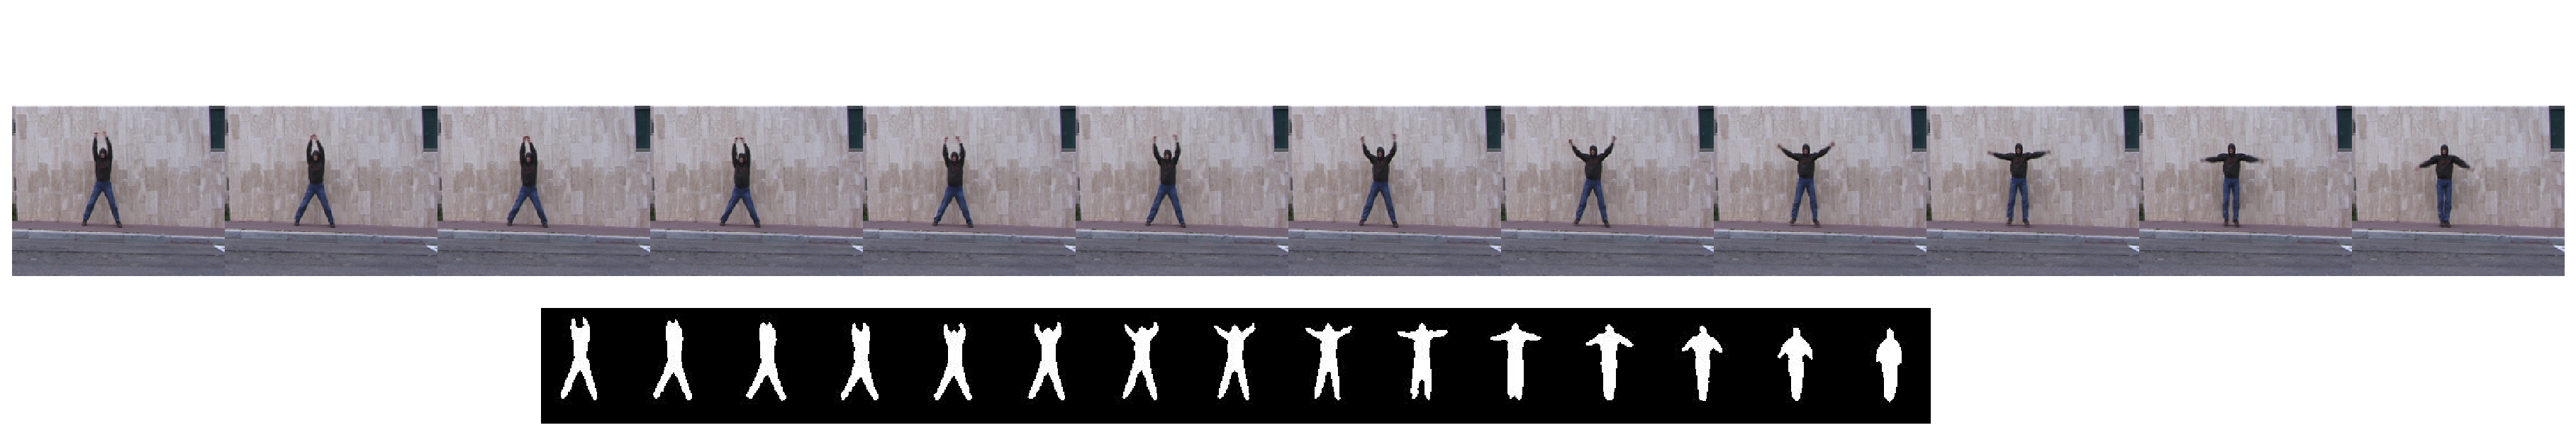
\includegraphics[width=1.0\textwidth]{figs/Proposal_fig5_RVQ_HMM_Weizmann_dataset}	
\caption{Sample images from the Weizmann dataset.}
\label{fig:Weizmann_sequence}
\end{figure}

In this chapter, we introduce our usage of RVQ for human action recognition \cite{2010_CNF_HMMRVQ_Aslam}.  The area of human action recognition has recently received a lot of attention.  A number of surveys are available on this topic \cite{1995_JNL_SURVEYmotion_Cedras, 1999_JNL_SURVEYmotion_Aggarwal, 1999_JNL_SURVEYmotion_Gavrila, 1999_REP_SURVEYmotion_Moeslund, 2001_JNL_SURVEYmotion_Moeslund, 2003_JNL_SURVEYiu_Buxton, 2003_JNL_SURVEYmotion_LWang, 2003_JNL_SURVEYbeh_Shah,2003_JNL_SURVEYaction_JWang, 2004_CNF_SURVEYaction_Aggarwal, 2004_JNL_SURVEYiu_Hu, 2004_CNF_SURVEYgait_Nixon, 2004_CNF_Survey3DshapeRetrieval, 2006_JNL_HumanMotion_Moeslund, 2007_JNL_HumanMotion_Poppe, 2008_CNF_SurveyHumanActivityRecognition_Ahad, 2010_JNL_SURVEYmotion_Ji}.  Bobick et al. \cite{2001_JNL_MotionTemplates_Bobick} introduced the notion of 2D templates of human action.  This was extended to 3D by Gorelick et al. \cite{2007_JNL_SpaceTimeShapes_Gorelick}.  Recently an approach based on kinematic features of 3D motion was used to recognize human action \cite{2010_JNL_ActionReconKinematic_Ali}.  Our approach to tackling this problem is similar to \cite{2007_JNL_SpaceTimeShapes_Gorelick} in the sense that extracted features are used for classification using a simple Euclidean distance measure.  

We use a four step approach:  

			\begin{figure}%[htp]
						
						\subfigure[Decoder codebooks.  With 2 code-vectors per stage, and 8 stages, a total of 256 reconstructed images are possible.  With 3 code-vectors per stage, a total of 6561 reconstructed images are possible.]
						{
							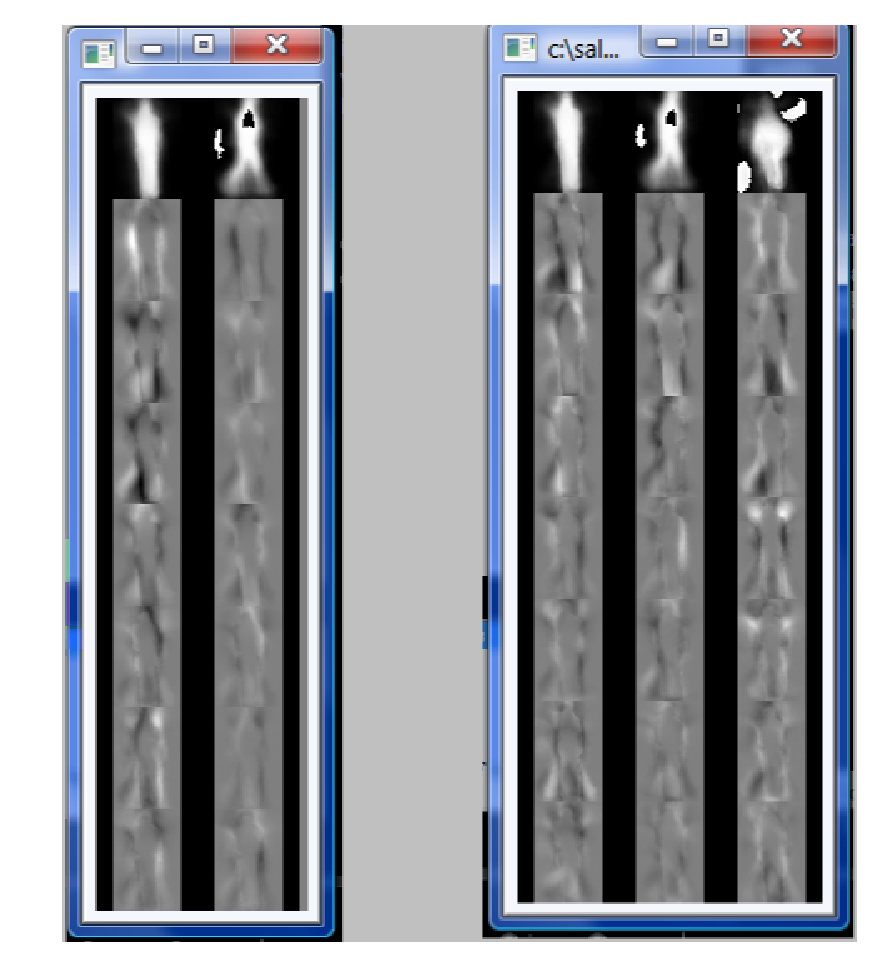
\includegraphics[width=.50\textwidth]{figs/Proposal_fig6a_RVQ_HMM_Weizmann_codebooks}
							\label{fig:Weizmann_codebooks}	
						}
						\hspace{1in}
						\subfigure[Image reconstruction using the decoder codebooks.]
						{
							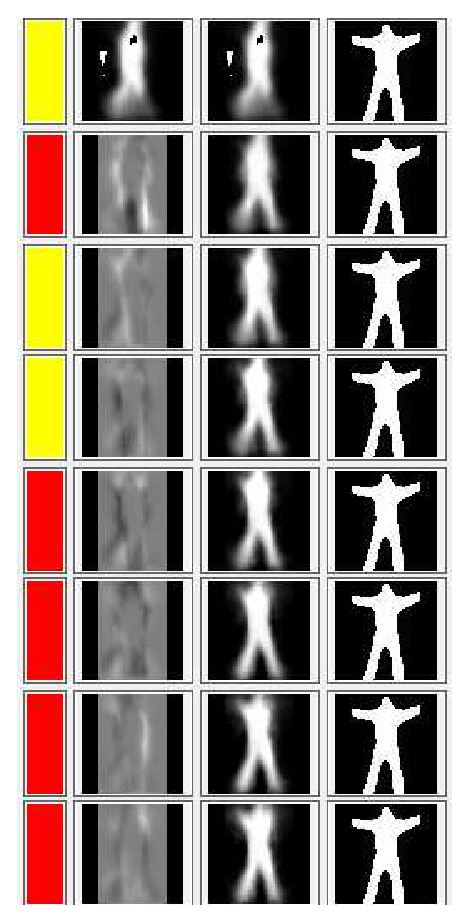
\includegraphics[width=0.25\textwidth]{figs/Proposal_fig6b_RVQ_HMM_Weizmann_reconstruction}
							\label{fig:Weizmann_reconstruction}	
						}
						\caption{Human action recognition, codebooks and reconstruction.} 
						\label{fig:Weizmann_codebooks_and_reconstruction}				
			\end{figure}
			
\begin{enumerate}			
\item In the first step, we separate the dataset shown in Figure~\ref{fig:Weizmann_sequence} into training and test images using the leave one out method \cite{2000_JNL_SURVEYprml_Jain}.  RVQ codebooks, shown in Figure~\ref{fig:Weizmann_codebooks}, are generated using this training set.  This one time offline step takes approximately 6 minutes for 2400 images on a Core2 Duo 2.5 GHz laptop.  

\item In the second step, a descriptor $x_i$ is generated for each of the $i$ training images using the decoder codebooks.  The first stage is weighted the most, followed by geometrically decreasing weights for the subsequent stages.  For $M$ code-vectors per stage and a total of $P$ stages, the descriptor, $x_i$ is a geometric sum given by,

\begin{equation}
x_i=\sum_{p=0}^{P-1}a_pM^{(P-1-p)}
\end{equation}

Notice that for 2 code-vectors per stage, the descriptor ranges from 0 to 255, and a single byte is required to represent an entire image.  These training image descriptors can be used for classification in a manner similar to the training image projections in PCA analysis.  The RVQ based descriptors or PCA based projections can be used to create class conditional densities.  These densities can then be used for classification using maximum likelihood, or maximum aposteriori methods.  The processing time to create training image descriptors is about 3 minutes.  However, it is also an offline step.  The processing time includes GUI related instructions as well as SQL Server database access times.

			\begin{figure}
						\centering	
						\subfigure[Our method \cite{2010_CNF_HMMRVQ_Aslam}]
						{
							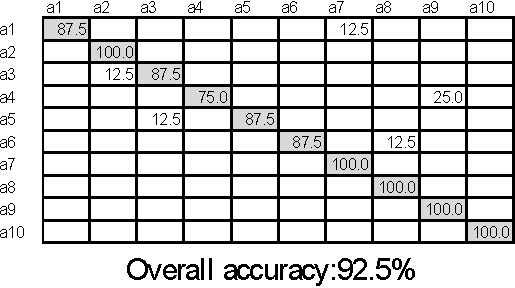
\includegraphics[width=.50\textwidth]{figs/Proposal_fig7a_RVQ_HMM_Weizmann_TabularResults_us}
							\label{fig:Weizmann_TabularResults_us}	
						}
						\subfigure[Gorelick et al. \cite{2007_JNL_SpaceTimeShapes_Gorelick}]
						{
							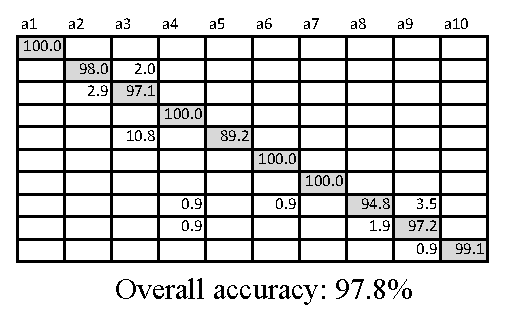
\includegraphics[width=0.45\textwidth]{figs/Proposal_fig7b_RVQ_HMM_Weizmann_TabularResults_gorelick}
							\label{fig:Weizmann_TabularResults_gorelick}	
						}
						\subfigure[Manor et al. \cite{2001_CNF_EventBasedAnalysisVideo_Manor}]
						{
							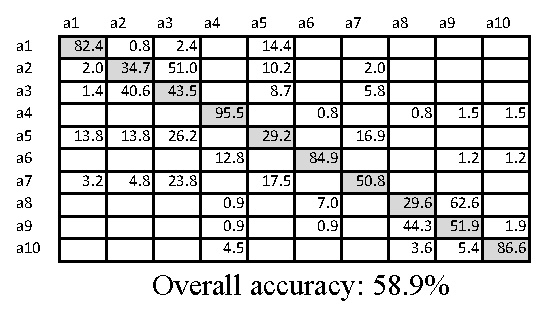
\includegraphics[width=0.50\textwidth]{figs/Proposal_fig7c_RVQ_HMM_Weizmann_TabularResults_manor}
							\label{fig:Weizmann_TabularResults_irani}	
						}
						\subfigure[Ali et al. \cite{2010_JNL_ActionReconKinematic_Ali}]
						{
							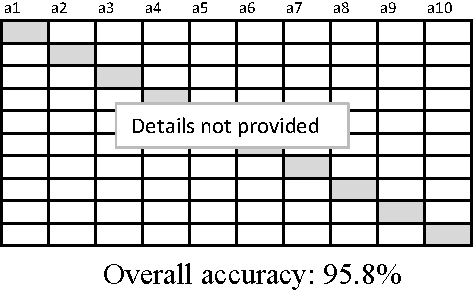
\includegraphics[width=0.45\textwidth]{figs/Proposal_fig7d_RVQ_HMM_Weizmann_TabularResults_shah}
							\label{fig:Weizmann_TabularResults_shah}	
						}												
						\caption{Human action recognition, action confusion matrix.} 
						\label{fig:Weizmann_TabularResults}				
			\end{figure}
						
\item In the third step, an HMM is trained on the descriptor evolution for every action sequence in the training set.  The 10 actions available are walk (a1), run (a2), skip (a3), jumping jacks (a4), jumping (a5), in-place jumping (a6), sideways motion (a7), waving with one hand (a8), waving with two hands (a9) and bending (a10).  There are a total of 8 users.  This step takes around 700 msec in Matlab.  All previous steps were executed in the C language.

\item In the fourth step, descriptor sequences are generated for the test images and tested against each HMM action model.  The model that best represents an action is picked.  This step is then repeated for all users in the database using the leave one out procedure.  This step takes 1.1 msec per frame in Matlab.   
\end{enumerate}

We compare our results in Figure~\ref{fig:Weizmann_TabularResults} with other researchers who have used the same database for exactly the same human action recognition purposes.  It may be noted that our results are based on using only 40\% of the training images.  The reason for not using the entire dataset is that each action has a different number of images in the database.  We have used an equal number of 25 images per action corresponding to half a second of video.  It is expected that if 1 second clips are used for all actions, our results will improve.  Unfortunately, at this point, this dataset does not have 1 sec clips for all actions.  



Our approach is based on using Hidden Markov models.  An HMM is given in Figure~\ref{fig:HMM}.  

	\begin{figure}			
		\includegraphics[width=1.0\textwidth]{figs/HMM}
		\caption{Discrete Hidden Markov Model (HMM), $N$ states, $M$ discrete observation symbols per state}
		\label{fig:HMM}
	\end{figure}






%@@@@@@@@@@@@@@@@@@@@@@@@@@@@@@@@@@@@@@@@@@@@@@@@@@
\chapter{RVQ: single target tracking}
\label{chap_RVQ_STT}	
%@@@@@@@@@@@@@@@@@@@@@@@@@@@@@@@@@@@@@@@@@@@@@@@@@@

%########################
\section{Introduction}
%########################
RVQ based target tracking involves XDR correspondence over time.  No prior assumptions are made about the target appearance model.  The following approach is used for every one of the $T$ targets tracked:

\begin{itemize}
	\item \textbf{Bootstrapping}
		\begin{enumerate}
			\item \textbf{Manual selection of target bounding box}.  A single bounding box is manually drawn around each of the $T$ targets of interest to initialize the tracking process.  		
			\item \textbf{Selection of several snippets from the target}.  $S$ smaller snippets with width $w_s$ and height $h_s$ , spaced 1 to 2 pixels apart in the x and y directions, are extracted from each of the $T$ targets.
			\item \textbf{Codebook training}.  $S$ snippets from $T$ targets obtained in the step above are used to train a single RVQ codebook, $C$.  The software flow for this training process is shown in Appendix~\ref{app:AppendixA}, Figure~\ref{fig:RVQ_sw_training}.
			\item \textbf{Compute XDRs for training snippets of target}.  $S$ training snippets per target are reconstructed using the trained codebook $C$.  The resulting $S$ XDR descriptors per target serve as $S$ observations per target that will be used as reference for correspondence and matching XDRs in subsequent frames.  The software flow for this process is shown in Appendix~\ref{app:AppendixA}, Figure~\ref{fig:RVQ_sw_testing}
		\end{enumerate}
	\item \textbf{Search for matching XDRs in subsequent images.}  
		\begin{enumerate}	
			\item \textbf{Compute XDRs}.  A window $W$ with width $snp_w$ equal to the training snippets is swept over a test image.  At every and XDR dsuch that the entire window is always contained inside the image.  Therefore, for a window with width $w$ and height $h$ is tested .  An XDR descriptor is obtained for every window position in the image such that the e  
			\item \textbf{Match XDR's}.
		\end{enumerate}
\end{itemize}


We keep the stage codevectors and so all images can be discarded (?)

%########################
\section{Motion model}
%########################
In most works, some assumption about constant motion or constant acceleration is made.  We make no assumptions about the motion that the target can take.  Moreover, it is difficult to make any assumptions about target motion if there is no prior information on camera motion.  We therefore choose to model motion as brownian motion.  This tracking method can handle:

\begin{enumerate}
\item arbitrary camera motion (translation and rotation)
\item arbitrary target motion (translation and rotation)
\item scale changes
\item lighting changes
\item pose (orientation) changes
\item structured noise
\item temporary occlusions
\end{enumerate}

Several gaussian distributions are used to handle these changes.  One distribution each is used to handle arbitrary translation in the horizontal direction, vertical direction, scale, rotation.  At every time step, predicted values are sampled from these distributions.  Each predicted value is warped to a standard window size and tested against the existing model.  The predicted value closest to the current model is selected as the next estimate and is used to update the model.  In PCA, the model is the eigenvectors, in RVQ, it's the stage codevectors and in TSVQ, it's the terminal codevectors.  


%########################
\newpage
\section{Employment of RVQ in tracking}
%########################


%########################
\newpage
\section{Observation model}
%########################

%########################
\section{Correspondence}
%########################
An XDR is a sequence of length $P$, i.e. a $P$-tuple, drawn from a finite alphabet $\{1, 2, \ldots M\}$.  The goal in tracking is to match $P$-tuples for a given target across frames.  Many methods can be used for this:

\begin{enumerate}
	\item \textbf{Distance in $R^P$}:  This method involves computing the Euclidean, Hamming or some other distance metric in $R^P$.  
	\item \textbf{Conversion to scalar value}: For $M$ code-vectors per stage and $P$ stages, the XDR can be converted through a geometric weighting to a scalar XDR, sXDR, using an invertible mapping sXDR$=\sum_{p=0}^{P-1}XDR(p)M^{(P-1-p)}$.  The reasoning behind this approach is that the first stage codevector should be given the highest weight, followed by monotonically decreasing weights for subsequent elements in the $p$-tuple.  The geometric weighting ensures an invertible mapping.
	\item Naive Bayes classifier:  In this approach, a Bayesian network is created over multiple XDR observations of a single target.  In order to avoid combinatorial complexity, a first order Markov assumption is made, as shown in Figure~\ref{fig:RVQ_bayesNet}.

\begin{figure}
\centering
\includegraphics[width=0.75\textwidth]{figs/RVQ_bayesNet.pdf}
\caption{A Bayesian network for a target XDR.  The XDR has $P$ elements.}
\label{fig:RVQ_bayesNet}
\end{figure}

	\item HMM:
\end{enumerate}


In this section, we track multiple targets using static codebooks and large blocks.
The following steps are followed:

\begin{figure}
\centering
\includegraphics[width=0.75\textwidth]{figs/Exp_GT1_input_RVQ_multi_target_snippets.pdf}
\caption{Training: six targets are manually selected from this training image and tracked simultaneously.  A single point in each target is clicked for initialization.  9 training snippets per target in the clicked pixel's 8-connected neighborhood are selected for RVQ training.}
\label{fig:Exp1_results_RVQ_input}
\end{figure}

\begin{enumerate}
	\item \textbf{Manual initialization}  Six targets in Figure~\ref{fig:Exp1_results_RVQ_input} are selected.  A single point in each target is clicked.  Nine 41x21 (height x width) pixel windows centered at that point and at all its 8-neighborhood pixels are selected for training RVQ codebooks.

\begin{figure}[h]
\centering
\includegraphics[width=0.45\textwidth]{figs/Exp_GT1_results_RVQ_codebooks.png}
\caption{TRAINING: Creating codebooks, in this case 8x4, i.e. 8 stages with 4 templates per stage}
\label{fig:Exp1_results_RVQ_codebooks}
\end{figure}


	\item \textbf{Training} An 8x4 RVQ is trained.  The trained DSSA codebooks are shown in  Figure~\ref{fig:Exp1_results_RVQ_codebooks}.  The first column codevectors remain relatively energetic up till 8 stages whereas in the other columns, after 4 stages, the codevectors are not very energetic (why ???).  Also, notice that all 4 codevectors in the first stage (top level) represent targets with different textures.  Since target 1 and target 4 in Figure~\ref{fig:Exp1_results_RVQ_input} are wearing shirts with similar hue and texture, they share a common top level codevector.  

 \begin{figure}
\centering	
\subfigure[Target 1]
{
\includegraphics[width=.47\textwidth]{figs/Exp_GT1_results_RVQ_target1_XDR.pdf}
\label{fig:Exp1_results_RVQ_target1_XDR}	
}
\subfigure[Target 2]
{
\includegraphics[width=0.47\textwidth]{figs/Exp_GT1_results_RVQ_target2_XDR.pdf}
\label{fig:Exp1_results_RVQ_target2_XDR}	
}
\subfigure[Target 3]
{
\includegraphics[width=.47\textwidth]{figs/Exp_GT1_results_RVQ_target3_XDR.pdf}
\label{fig:Exp1_results_RVQ_target3_XDR}	
}
\subfigure[Target 4]
{
\includegraphics[width=0.47\textwidth]{figs/Exp_GT1_results_RVQ_target4_XDR.pdf}
\label{fig:Exp1_results_RVQ_target4_XDR}	
}	
\subfigure[Target 5]
{
\includegraphics[width=.47\textwidth]{figs/Exp_GT1_results_RVQ_target5_XDR.pdf}
\label{fig:Exp1_results_RVQ_target5_XDR}	
}
\subfigure[Target 6]
{
\includegraphics[width=0.47\textwidth]{figs/Exp_GT1_results_RVQ_target6_XDR.pdf}
\label{fig:Exp1_results_RVQ_target6_XDR}	
}
\caption{TESTING on training image: XDR evolution for all tracked targets, 9 snippets per target.  Targets 1 and 4 are similar and therefore share a common top-level code-vector.  Target 2 also shares a common code-vector with targets 1 and 4 since there is one less templates per stage than number of targets.  All other targets have unique top level code-vectors.  Also, all targets have one or two second-level codevectors.}		
\label{fig:Exp1_results_RVQ_XDRevolution}				
\end{figure}

	\begin{enumerate}
	\item \textbf{Generate XDRs for training snippets}.   The next step is to use the codebooks to generate XDRs for the training snippets.  The resulting XDRs are shown in Figure~\ref{fig:Exp1_results_RVQ_XDRevolution}.  As mentioned above, Figure~\ref{fig:Exp1_results_RVQ_target1_XDR} and Figure~\ref{fig:Exp1_results_RVQ_target4_XDR} show that targets 1 and 4 both map to the left-most top-level codevector.  Also, since there are a total of 6 targets, another target has to share a top-level codevector with another target.  This happens to be target 2 that also shares the same top-level codevector with targets 1 and 4.  This is shown in Figure~\ref{fig:Exp1_results_RVQ_target4_XDR}.  However, this creates a large reddish residual which is evident in the left-most second-stage codevector, to which this target maps to.  The remaining 3 targets have their own top-level stage codevectors, and this can be seen in the codebooks as well as Figures~\ref{fig:Exp1_results_RVQ_target3_XDR}, \ref{fig:Exp1_results_RVQ_target5_XDR} and \ref{fig:Exp1_results_RVQ_target6_XDR}.  

	
\begin{figure}
\centering	
\subfigure[All 54 snippets, 9 for target 1, 9 for target 2, and so on are tested against every HMM model and log likelihood is computed.]
{
\includegraphics[width=.47\textwidth]{figs/Exp_GT1_results_RVQ_HMMtrgLikelihoods.pdf}
\label{fig:Exp1_results_RVQ_HMMtrgLikelihoods}	
}
\subfigure[Confusion matrix derived from log likelihood.  98-100\% classification accuracy is obtained depending on HMM initialization]
{
\includegraphics[width=0.47\textwidth]{figs/Exp_GT1_results_RVQ_HMMconfusionMatrix.pdf}
\label{fig:Exp1_results_RVQ_HMMconfusionMatrix}	
}	
\caption{TESTING on training image: Confusion matrix.}
\label{fig:Exp_GT1_results_RVQ_HMMtestingOnTrgSnippets}				
\end{figure}

	\item \textbf{Train HMM on training XDRs}.  In order to carry out detection in subsequent frames, one 4-stage HMM per target is trained on the XDR evolution.  Classification accuracy on the XDRs used to generate the HMMs is 100\%.  The confusion matrix for this is shown in Figure~\ref{fig:Exp1_results_RVQ_HMMconfusionMatrix}.
\end{enumerate}
	\item \textbf{Testing on training image}.  Before testing is done on subsequent test images, we carry out testing on the training image.  This is done in one of two ways

\begin{figure}
\centering	
\subfigure[Scaled reconstruction SNR overlaid on training image (2D)]
{
\includegraphics[width=.47\textwidth]{figs/Exp_GT1_results_RVQ_FN0_cor2D.pdf}
\label{fig:Exp1_results_RVQ_cor2D}	
}
\subfigure[Scaled reconstruction SNR overlaid on training image (3D)]
{
\includegraphics[width=0.47\textwidth]{figs/Exp_GT1_results_RVQ_FN0_cor3D.pdf}
\label{fig:Exp1_results_RVQ_cor3D}	
}
\subfigure[Number of stages required during reconstruction for monotonically increasing SNR]
{
\includegraphics[width=0.47\textwidth]{figs/Exp_GT1_results_RVQ_FN0_stg.pdf}
\label{fig:Exp1_results_RVQ_stg}	
}
\subfigure[Areas with max stages and high reconstruction SNR]
{
\includegraphics[width=0.47\textwidth]{figs/Exp_GT1_results_RVQ_FN0_stgsnr.pdf}
\label{fig:Exp1_results_RVQ_stgcor}	
}		
\caption{TESTING on training image: scaled reconstruction SNR and number of stages}										
\label{fig:ECE8833a_trainingImage}				
\end{figure}

\begin{enumerate}
	\item \textbf{Spatial domain}:  In Figure~\ref{fig:Exp1_results_RVQ_cor2D} and \ref{fig:Exp1_results_RVQ_cor3D}, spatial domain reconstruction SNR is shown for the entire image.  The number of stages required for monotonic increase in reconstruction SNR is shown in Figure~\ref{fig:Exp1_results_RVQ_stg}.    Figure~\ref{fig:Exp1_results_RVQ_stghist} displays a histogram of stages used during reconstruction of every snippet in the training image.  It is clear that very few reconstructions use all stages.  For areas that have low stage reconstruction, low reconstruction SNR is an indication that these areas are not in the training set, as in the sky while areas of high SNR indicate that similar regions are part of the training set, as in the grassy areas.  However, as explained in Section~\ref{Sec_stages_vs_reconstructionSNR}, we test for target presence only in areas of maximum stages and high reconstruction SNR.  The result of this operation can be seen in Figure~\ref{fig:Exp1_results_RVQ_stgcor}.  It is clear that all six targets are correctly detected in the training image.  
	\item \textbf{HMM testing on XDR evolution}:
\end{enumerate}

\end{enumerate}


\begin{figure}
\centering
\includegraphics[width=0.45\textwidth]{figs/Exp_GT1_results_RVQ_stghist.pdf}
\caption{TESTING on training image: histogram of number of stages required during reconstruction for monotonically increasing SNR}
\label{fig:Exp1_results_RVQ_stghist}
\end{figure}






%########################
\section{Comparison with PCA}
%########################



%########################
\section{Comparison with TSVQ}
%########################


%@@@@@@@@@@@@@@@@@@@@@@@@@@@@@@@@@@@@@@@@@@@@@@@@@@
\chapter{RVQ: multi-target tracking}
\label{chap_RVQ_MTT}	
%@@@@@@@@@@@@@@@@@@@@@@@@@@@@@@@@@@@@@@@@@@@@@@@@@@

%########################
\section{Maintaining multiple codebooks}
%########################

%@@@@@@@@@@@@@@@@@@@@@@@@@@@@@@@@@@@@@@@@@@@@@@@@@@
\chapter{Conclusions}
\label{chap_Conclusions}	
%@@@@@@@@@@@@@@@@@@@@@@@@@@@@@@@@@@@@@@@@@@@@@@@@@@


%@@@@@@@@@@@@@@@@@@@@@@@@@@@@@@@@@@@@@@@@@@@@@@@@@@
\appendix{Appendices}
\label{app:AppendixA}
%@@@@@@@@@@@@@@@@@@@@@@@@@@@@@@@@@@@@@@@@@@@@@@@@@@


%########################
\newpage
\section{RVQ software flow diagram}
\label{app:RVQ_sw_flowDiagram}	
%########################

\begin{figure}[htp]
	\centering	
	\subfigure[RVQ training]
	{
		\includegraphics[width=1.0\textwidth]{figs/RVQ_software_training.pdf}
		\label{fig:RVQ_software_training}	
	}
	\subfigure[RVQ testing]
	{
		\includegraphics[width=0.8\textwidth]{figs/RVQ_software_testing.pdf}
		\label{fig:RVQ_software_testing}	
	}		
	\caption{RVQ training and testing, software flow}
	\label{fig:RVQ_testing}	
\end{figure}










%##############################################################################################################
\end{Body}
\begin{EndMatter}
\references% Generates the bibliography page
\end{EndMatter}
\end{document}

%##############################################################################################################
%##############################################################################################################

